

\graphicspath{{./ch_adptv_msmnt_magnetometry/figures/}}


\chapter{ Optimized quantum sensing with a single electron spin
using real-time adaptive measurements}
\label{ch:AMM}


{\renewcommand{\thefootnote}{}\footnote{This chapter has been submitted to
    {\em Nature Nanotechnology} (2015).}}

\begin{center} 
    \vspace{-1cm} {C.~Bonato, M.S.~Blok, H.T. ~Dinani, D.W. ~Berry, M.L. ~Markham, D.J. ~Twitchen  and R.~Hanson} 
\end{center}


\vspace{-0.5cm} 
Quantum sensors based on single solid-state spins promise a unique combination of sensitivity and spatial resolution1-20. The key challenge in sensing is to achieve minimum estimation uncertainty within a given time and with a high dynamic range. Adaptive strategies have been proposed to achieve optimal performance but their implementation in solid-state systems has been hindered by the demanding experimental requirements. Here we realize adaptive d.c. sensing by combining single-shot readout of an electron spin in diamond with fast feedback. By adapting the spin readout basis in real time based on previous outcomes we demonstrate a sensitivity in Ramsey interferometry surpassing the standard measurement limit. Furthermore, we find by simulations and experiments that adaptive protocols offer a distinctive advantage over the best-known non-adaptive protocols when overhead and limited estimation time are taken into account. Using an optimized adaptive protocol we achieve a magnetic field sensitivity of $6.1\pm 1.7$ nT Hz$^{-\frac{1}{2}}$ over a wide range of 1.78 mT. These results open up a new class of experiments for solid-state sensors in which real-time knowledge of the measurement history is exploited to obtain optimal performance.


\clearpage

\section{Introduction}
Quantum sensors have the potential to achieve unprecedented sensitivity by exploiting control over individual quantum systems1,2. As a prominent example, sensors based on single electron spins associated with Nitrogen-Vacancy (NV) centers in diamond capitalize on the spin?s quantum coherence and the high spatial resolution resulting from the atomic-like electronic wave function3,4. Pioneering experiments have already demonstrated single-spin sensing of magnetic fields5-7, electric fields8, temperatures9,10 and strain11. NV sensors may therefore have a revolutionary impact on biology12-15, nanotechnology16-18 and material science19,20. 

A spin-based magnetometer can sense a d.c. magnetic field \textit{B} through the Zeeman shift $E_z=\hbar \gamma B = \hbar 2 \pi f_B$ ($\gamma$ is the gyromagnetic ratio and $f_B$ the Larmor frequency) between two spin levels $\ket{0}$ and $\ket{1}$. In a Ramsey interferometry experiment, a superposition state  $\frac{1}{\sqrt{2}}$($\ket{0}$ + $\ket{1}$), prepared by a $\pi$/2 pulse, will evolve to $\frac{1}{\sqrt{2}}$($\ket{0}$ + $e^{i\varphi}\ket{1}$)   over a sensing time \textit{t}. The phase $\varphi = 2 \pi f_B t$ can be measured by reading out the spin in a suitable basis, by adjusting the phase $\vartheta$ of a second $\pi$/2 pulse.


For a Ramsey experiment that is repeated with constant sensing time \textit{t} the uncertainty $\sigma_{f_B}$ decreases with the total sensing time \textit{T} as 1/(2 $\pi \sqrt{tT}$) (standard measurement sensitivity, SMS).  However, the field range also decreases with \textit{t} because the signal is periodic, creating ambiguity whenever $|2\pi f_B t| > \pi $. This results in a dynamic range bounded as  $f_{B,max}$/$\sigma_{f_B}  \le \pi \sqrt{T/t}$.  Recently, it was discovered that the use of multiple sensing times within an estimation sequence can yield a scaling of $\sigma_{f_B}$ as 1/\textit{T}, resulting in a vastly improved dynamic range: $f_{B,max}$/ $\sigma_{f_B} \le  \pi T $/$ \tau_{min}$, where $\tau_{min}$ is the shortest sensing time used. A major open question is whether adaptive protocols, in which the readout basis is optimized in real time based on previous outcomes, can outperform non-adaptive protocols. While scaling beating the standard measurement limit has been reported with non-adaptive protocols22,23, feedback techniques have only recently been demonstrated for solid-state quantum systems24-26 and adaptive sensing protocols have so far remained out of reach.


Here we implement adaptive d.c. sensing with a single-electron spin magnetometer in diamond by exploiting high-fidelity single-shot readout and fast feedback electronics (Fig.\,\ref{fig:amm-fig1}). We demonstrate a sensitivity beyond the standard measurement limit over a large field range. Furthermore, we investigate through experiments and simulations the performance of different adaptive protocols and compare these to the best known non-adaptive protocol. Although the non-adaptive protocol improves on the standard measurement limit for sequences with many detections we find that the adaptive protocols perform better when overhead time for initialization and readout is taken into account. In particular, the adaptive protocols require shorter sequences to reach the same sensitivity, thus allowing for sensing of signals that fluctuate on shorter timescales.

\begin{figure*}
	\centering
	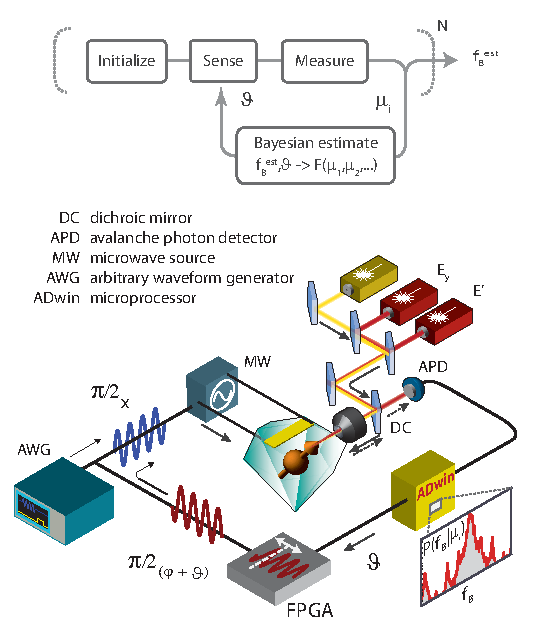
\includegraphics{Fig_1_setup}
	\caption{\label{fig:amm-fig1} \textbf{Experiment concept and apparatus.} The adaptive frequency estimation protocol consists of a sequence of initialization, sensing, measurement operations. After each measurement run, the outcome $\mu$ is used to update the estimate of the frequency $f_B$, which is then used to optimize the sensing parameters for the following run. Experimentally, the frequency estimation and adaptive calculation of the phase are performed in real-time by a microprocessor.}
\end{figure*}

Our magnetometer employs two spin levels of a single NV center electron in isotopically purified diamond (0.01 \% $^{13}C$). We exploit resonant spin-selective optical excitation, at a temperature of 8 K, for high-fidelity initialization and single-shot readout!!!TODO ADD REF!! (Fig.\,\ref{fig:amm-fig2}a). Microwave pulses, applied via an on-chip stripline, coherently control the electron spin state. From Ramsey experiments, we measure a spin dephasing time of $T_2^* = (96 \pm 2) \mu$s (Fig.\,\ref{fig:amm-fig2}b). In order to characterize the performance of different sensing protocols in a controlled setting, the effect of the external field is implemented as an artificial frequency detuning, by adding $\varphi = 2 \pi f_B t$ to the phase $\vartheta$  of the final $\pi$/2-pulse. To achieve high sensitivity in a wide field range we use an estimation sequence consisting of \textit{N} different sensing times21-23,28, varying as $\tau_n = 2^{(N-n)} \tau_{min}$ ( \textit{n} = 1..\textit{N}). The value of $\tau_{min}$ sets the range; we take $\tau_{min}$ = 20 ns, corresponding to a range |$f_B$| < 25  MHz, equivalent to |\textit{B}| < 0.89 mT for $\gamma = 2 \pi \times 28$ MHz mT$^{-1}$.

\begin{figure*}
	\centering
	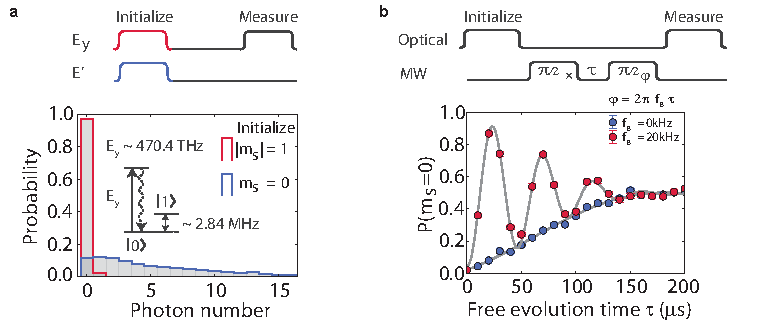
\includegraphics{Fig_2_ssro_ramsey}
	\caption{\label{fig:amm-fig2} \textbf{Single shot readout and Ramsey.} (a) The experiment is performed using the states $\ket{0} = \ket{m_s = 0}$,$\ket{1} = \ket{m_s = -1}$ of the  electronic spin of a NV centre in diamond. The electronic spin is readout by resonant optical excitation and photon counting27: detection of luminescence photons corresponds to detection of the $\ket{0}$ state. We plot the probability of detecting a photon after initializing either in $\ket{0}$ or $\ket{1}$. The readout fidelities for the states $\ket{0}$ (outcome 0) and $\ket{1}$  (outcome 1) are $F_0 = 0.88 \pm 0.02$, $F_1 = 0.98 \pm 0.02$, respectively. (b) Each measurement run consists of a Ramsey experiment, in which the phase accumulated over time by a spin superposition during free evolution is measured. The measurement basis rotation is controlled by the phase $\vartheta$ of the final $\pi$/2-pulse. From the measured phase, we can extract the frequency $f_B$, corresponding to an energy shift between the levels $\ket{0}$ and $\ket{1}$ given by an external field (magnetic field, temperature, strain…). Here, to test the performance of different protocols, we set $f_B$ as an artificial detuning, set by the microprocessor by adding $\varphi = 2 \pi f_B t$ to the phase $\vartheta$ (Supplementary Figure !!!TODO ADD REF!!!!!).}
\end{figure*}

The key idea of adaptive magnetometry is that for each Ramsey experiment the measurement basis is chosen based on the previous measurement outcomes such that the uncertainty in the frequency estimation is minimized (Fig.\,\ref{fig:amm-fig1}). After every Ramsey experiment, the outcome is used to update a frequency probability distribution $P(f_B)$ according to Bayes’ rule, taking measured values for detection fidelity and coherence time into account (Methods). The current estimate of $P(f_B)$ is then used to calculate the phase $\vartheta$ of the final $\pi$/2-pulse which allows for best discrimination between different possible magnetic field values in the next Ramsey experiment28. In our experiment, this process is realized by a microprocessor, which receives the measurement outcome, performs the Bayesian estimate, calculates the  phase $\vartheta$ and subsequently sends a digital signal to a field-programmable gate array (FPGA) to adjust the phase of the final $\pi$/2-pulse accordingly (Fig.\,\ref{fig:amm-fig1}).

To reduce the undesired effects of quantum projection noise and imperfect readout fidelity we perform $M_n$ Ramsey experiments21 for each sensing time $\tau_n$, with  $M_n = G + F (n-1)$. Here \textit{G} and \textit{F} can be chosen to optimize the performance of the protocol. For the short sensing times (large \textit{n}), corresponding to the measurements that make the largest distinction in frequency (and where an error is therefore most detrimental), we  perform the most Ramsey experiments. We will compare several protocols that differ in the strategy of adaptive phase choice. As a first example, we consider a protocol where the phase $\vartheta$ is adjusted each time the sensing time is changed; we name this “limited-adaptive” protocol. 

\begin{figure*}
	\centering
	\includegraphics[height=12.5cm]{Fig_3_protocol}
	\caption{\label{fig:amm-fig3} \textbf{High dynamic-range adaptive magnetometry.} Limited-adaptive protocol, in the case of one Ramsey experiment per sensing time (\textit{G} = 1, \textit{F} = 0). In each step, the current frequency probability distribution $P(f_B)$ is plotted (solid black line), together with conditional probabilities $P(\mu|f_B)$ for the measurement outcomes $\mu$ = 0 (red shaded area) and $\mu$=1 (blue shaded area). After each measurement,  $P(f_B)$ is updated according to Bayes’ rule. The detection phase $\vartheta$ of the Ramsey experiment is set to the angle which attains the best distinguishability between peaks in the current frequency probability distribution $P(f_B)$. Ultimately, the protocol converges to a single peak in the probability distribution, which delivers the frequency estimate.}
\end{figure*}

An example of the working principles of the limited-adaptive protocol is illustrated in Fig.\,\ref{fig:amm-fig3}, for an estimation sequence comprising $N = 3$ sensing times and one measurement per sensing time (\textit{G} = 1, \textit{F} = 0). We start with no information over $f_B$, corresponding to a uniform probability density $P(f_B )$ (solid black line).  For the first Ramsey experiment, the sensing time is set to $4 \tau_{min}$. $P(f_B)$ is updated depending on the measurement outcome. For example, the outcome 1 indicates maximum probability for the values $f_B = \pm 6.25, \pm 18.75$ MHz, and minimum probability for $f_B = 0, \pm 12.5, \pm 25$ MHz. This indeterminacy in the estimation originates from the fact that, for this sensing time, the acquired phase spans the range [-4$\pi$, 4$\pi$], wrapping multiple times around the [-$\pi$, $\pi$] interval. The sensing time is then decreased to $2 \tau_{min}$. Given the current $P(f_B)$ for outcome 1 (black curve), the filter functions that would be applied to $P(f_B)$ after the Bayesian update for detection outcomes 0 and 1 are represented, respectively, by the light red and blue areas. For $\vartheta = - /pi$/2, maximum distinguishability is ensured: outcome 0 would select the peaks around $f_B$ = -6.25, +18.75 MHz, while outcome 1 would select the peaks around $f_B$ = -18.75, +6.25 MHz. The same process is then repeated, decreasing the sensing time to  $\tau_{min}$. The remaining uncertainty, corresponding to the width of the resulting peak in $P(f_B)$, is set by the longest sensing time $4 \tau_{min}$. 

\begin{figure*}
	\centering
	\includegraphics{Fig_4_Pfb_dynamicrange}
	\caption{\label{fig:amm-fig4} \textbf{Frequency dependence of uncertainty.} (a)-(b) Frequency estimate example, for (\textit{G} =  5, \textit{F} = 7). We set a fixed artificial detuning $f_B$ = 2 MHz and run different instances of the limited-adaptive frequency estimation protocol, with increasing \textit{N}. The resulting probability density $P(f_B)$ is averaged over 101 repetitions. (c) Holevo variance as a function of the frequency $f_B$ for \textit{N} = 2, 4 (limited-adaptive protocol, \textit{G} = 5, \textit{F} = 7). We vary $f_B$ by adjusting the phase of the final $\pi$/2-pulse. Solid lines correspond to numerical simulations, performed with 101 repetitions per frequency point and experimental parameters for fidelity and dephasing. Experimental points (triangular shape), were acquired with 101 repetitions each. Error bars (one standard deviation) are calculated by bootstrap analysis.}
\end{figure*}

Figure \,\ref{fig:amm-fig4}b shows the probability density yielded by experimental runs of the limited-adaptive protocol with different numbers of sensing times \textit{N} = 1,3,5,7,9. Here,  $f_B$ = 2 MHz, and each estimation sequence is repeated 101 times, with \textit{G} = 5, \textit{F} = 7. For increasing \textit{N}, the width of the distribution becomes more narrowly peaked around the expected value of 2 MHz, while the wings of distribution are strongly suppressed. 

To verify that the protocol works over a large dynamic range, we measure the uncertainty as a function of detuning $f_B$. To account for the periodic nature of phase we use the Holevo variance $V_H = (|<e^{i2 \pi f_B^{est} \tau_{min}}>|)^2 - 1$ as a measure of the uncertainty. We estimate  $f_B^{est}$ by taking the mean of the probability density $P(f_B)$ resulting from a single run of the protocol. A fixed initial phase ($\vartheta$ = 0 in our experiments) results in a specific dependence of the variance on the magnetic field. For example, for \textit{N} = 2, only four measurement outcomes are possible $\{$ 00, 01, 10, 11 $\}$, corresponding to $f_B$ = 0, -25, -12.5, +12.5 MHz, respectively. These specific detunings can be measured with the highest accuracy since they correspond to measurements of an eigenstate of our quantum sensor at the end of the Ramsey experiment, while for other frequencies larger statistical fluctuations will be found due to spin projection noise. Figure \,\ref{fig:amm-fig4}c shows $V_H$ as a function of detuning for the parameters \textit{G} = 5, \textit{F} = 7. Both the experimental data (dots) and the numerical simulation (solid lines) confirm the expected periodic behavior.

We now use our adaptive sensing toolbox to compare different sensing protocols by investigating the scaling of $\eta^2 = V_H T$, averaged over different detunings, as a function of the total sensing time \textit{T}. First, we will ignore the overhead time due to spin initialization and readout. 

We compare the limited-adaptive protocol to the best known non-adaptive protocol and to an optimized adaptive protocol. In the non-adaptive protocol 21-23, the readout phase for the $m^{th}$ Ramsey experiment is always set to $\vartheta_{n,m} = \frac{m\pi}{M_n}$  ( \textit{m} = 1..$M_n$). In the optimized adaptive protocol29,30, the phase $\vartheta$ is updated before each Ramsey and, additionally, a phase $\vartheta_{n,m}^{incr}$ that depends only on the current values of \textit{n},\textit{m} and the last measurement outcome $\mu_{n,m}$, is added. This additional $\vartheta_{n,m}^{incr}$ is determined by a numerical minimization of the Holevo variance, via swarm-optimization techniques, taking experimental parameters into account. A detailed description of all protocols is reported in Supplementary Tables !! TO DO ADD REF!!!.

We plot experimental data for the sensitivity scaling for the three protocols in Fig.\,\ref{fig:amm-fig5}a alongside simulations using known experimental parameters. In these graph, the SMS limit corresponds to a constant $V_H T$; any scaling behavior with a negative slope thus improves beyond the SMS.

\begin{figure*}
	\centering
	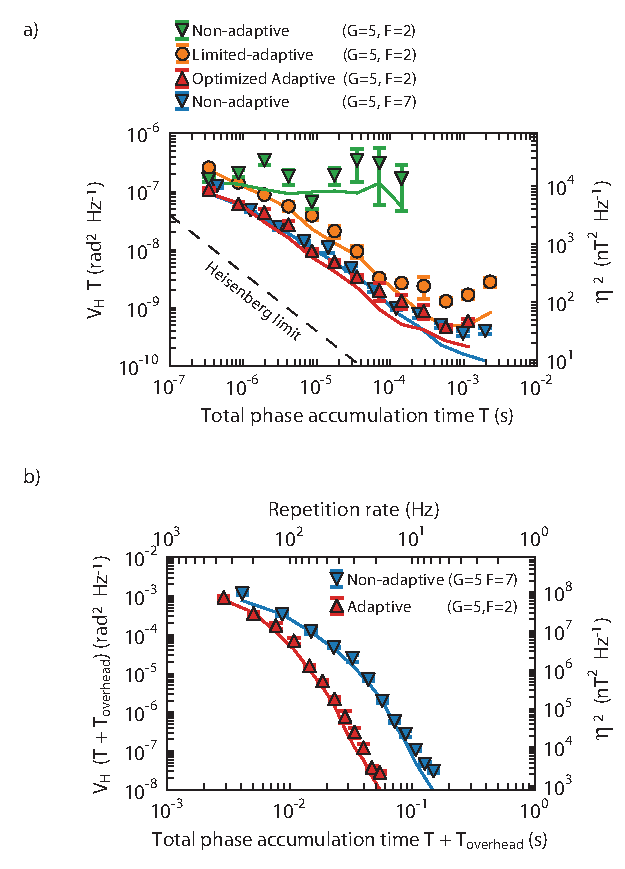
\includegraphics{Fig_5_scaling}
	\caption{\label{fig:amm-fig5} \textbf{Scaling of sensitivity as a function of total time.} (a) The three protocols are compared by plotting $\eta^2 - V_H T$  as a function of the total sensing time \textit{T} (not including spin initialization and readout). For (\textit{G} = 5, \textit{F} = 2) the non-adaptive protocol (green triangles) is bound to the SMS limit, while for both the limited-adaptive (orange circles) and the optimized adaptive (red triangles) protocols $\eta^2$ scales close to 1/\textit{T}. The sensitivity of the limited-adaptive protocol is, however, worse than the optimized-adaptive one. When increasing the number of Ramsey experiments per sensing time to (\textit{G} = 5, \textit{F} = 7), the non-adaptive protocol (blue triangles) reaches Heisenberg-like scaling, with a sensitivity comparable to the optimized adaptive protocol for (\textit{G}=5, \textit{F}=2). (b) By including spin initialization and readout durations, the superiority of the optimized adaptive protocol (red triangles), which requires less Ramsey runs per sensing time (smaller \textit{F}, \textit{G}) to reach 1/\textit{T} scaling, is evidenced. The optimized adaptive protocol can estimate magnetic fields with a repetition rate of 20 Hz, with a sensitivity more than one order of magnitude better than the non-adaptive protocol. All data are taken with 700 repetitions per data-point. In both plots, error bars corresponding to one standard deviation of the results are obtained using the bootstrap method.}
\end{figure*}


We observe that, for the setting (\textit{G} = 5, \textit{F} = 2), the non-adaptive protocol reaches only the SMS limit, while both adaptive protocols yield $V_H T$ scaling close to 1/\textit{T}. When the number of measurements per interaction time is increased to (\textit{G} = 5, \textit{F} = 7) the non-adaptive protocol also shows sub-SMS scaling (Fig.\,\ref{fig:amm-fig5}a, blue line). We find this behavior to be quite general: both adaptive and non-adaptive protocols can reach 1/\textit{T} scaling, but the adaptive protocols require fewer measurements (Supplementary Figures !!TODO: ADD REF!!!). By comparing the best non-adaptive and the best adaptive protocol, we find that they reach the same sensitivity of (6.1 $\pm$ 1.7) nT Hz$^{-\frac{1}{2}}$ when the longest sensing time reaches $T_2^*$. The non-adaptive protocol however, requires significantly more measurements (611) than the adaptive protocol (221).


The advantage of adaptive measurements becomes clear when the initialization and readout times (overhead) are taken into account (Fig \,\ref{fig:amm-fig5}b). Since the time required to compute the controlled phase is similar to the initialization time, the two operations can be performed simultaneously, with no additional overhead required by the adaptive protocol (Methods). While the two best protocols still achieve similar minimum sensitivities, the optimized adaptive protocol requires significantly less measurement time. At any fixed measurement time, the adaptive protocol estimates the magnetic field more accurately, allowing a higher repetition rate for the estimation sequences. This is advantageous in the realistic situation that the magnetic field to be estimated is not static: in this case, the estimation time is required to be shorter than the timescale of the fluctuations. Our data shows that at an estimation repetition rate of 20 Hz, the non-adaptive protocol can estimate a magnetic field with an sensitivity $\eta$ = (749 $\pm$ 35) nT Hz$^{-\frac{1}{2}}$, while the optimized-adaptive protocol yields $\eta$ = (47 $\pm$ 2) nT Hz$^{-\frac{1}{2}}$.

While the record sensitivity reported here is enabled by single-shot spin readout at low temperature, adaptive techniques can prove valuable also in experiments at room temperature23 where spin-dependent luminescence intensity under off-resonant excitation is typically used to measure the electronic spin. By averaging the signal over multiple repetitions an arbitrarily high readout fidelity can be achieved (\textit{F} = 0.99 for 50,000 repetitions23). Interestingly, we find that the benefits given by adaptive techniques persist also in case of lower readout fidelities and that the combination of adaptive techniques and optimization of the number of readout repetitions yields a significant improvement (Supplementary Figure !!!TODO: ADD REF!!!).

In conclusion, by combining high-fidelity single-shot readout at low temperature with a single electron spin sensor and fast electronics, we achieve an unprecedented d.c. sensitivity of (6.1 $\pm$ 1.7) nT Hz$^{-\frac{1}{2}}$ with a repetition rate of 20 Hz. Another relevant figure of merit for sensors is the ratio between the range and the sensitivity; the best value found in this work ($B_{max}$/$\eta \sim 1.5 \cdot 10^5 $Hz$^{\frac{1}{2}}$) improves on previous experiments by two orders of magnitude22,23. Furthermore, we found that the best known adaptive protocol outperforms the best known non-adaptive protocol when overhead is taken into account. These insights can be extended to other quantum sensors and to the detection of different physical quantities such as temperature and electric fields. A remaining open question is whether this adaptive protocol is optimal; perhaps further improvements are possible by taking into account the full measurement history. In a more general picture, the adaptive sensing toolbox demonstrated in this work will enable exploration of the ultimate limits of quantum metrology and may lead to practical sensing devices combining high spatial resolution, sensitivity, dynamic range and repetition rate.



\section{Methods}
M


%\bibliography{adptv_msmnt_cntrl}
